\documentclass[11pt]{article}
\topmargin -.25in
\oddsidemargin 0in
\textwidth 6.5in
\textheight 9in
\def\v{\vspace{11pt}}
\def\d{\displaystyle}
\pagestyle{empty}
\usepackage{graphics,amsmath,amssymb,ulem,tikz}
\usetikzlibrary{arrows.meta} 

\begin{document}
\centerline {\bf \large Quiz \# 4}
\v

\noindent Math 118 \hfill Names: \rule{2in}{.25mm}

\noindent Instructor: \rule{2in}{.25mm} \hfill \rule{2in}{.25mm}

\noindent Fall 2025 \hfill \rule{2in}{.25mm}

\hfill \rule{2in}{.25mm}

\v

\noindent To receive full credit you must show all work and provide clear, complete explanations.  Use of books, notes, calculators, etc.\ is not permitted.  

\begin{enumerate}
    \item (6 points) Use the given graphs of $f$ and $g$ to evaluate the expressions.
        \begin{center}
        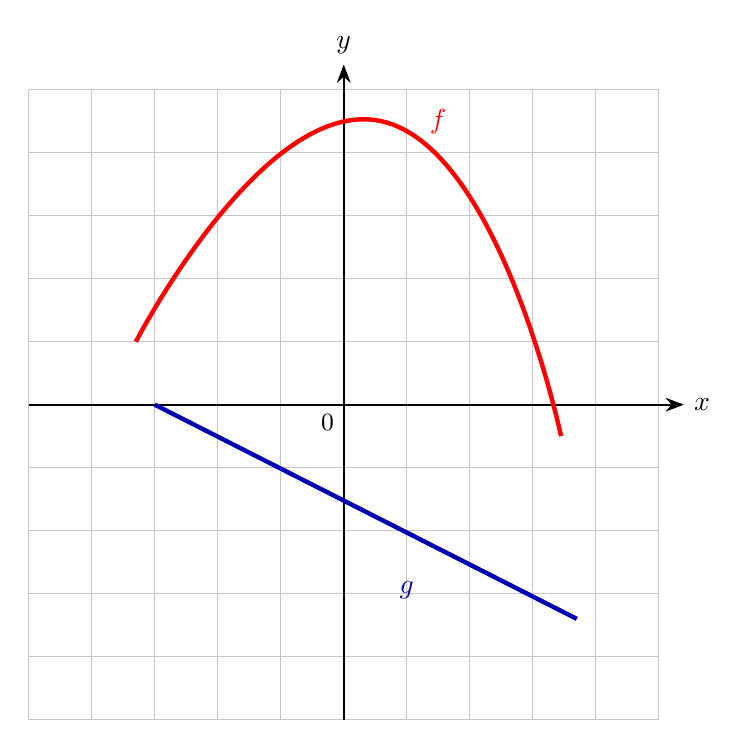
\begin{tikzpicture}[scale=0.8,>=Stealth]
            % grid
            \draw[step=1cm, very thin, gray!45] (-5,-5) grid (5,5);

            % axes
            \draw[->, thick] (-5,0) -- (5.4,0) node[right] {$x$};
            \draw[->, thick] (0,-5) -- (0,5.4) node[above] {$y$};
            \node[below left] at (0,0) {\small $0$};

            % f (red)
            \draw[ultra thick, red]
                plot[smooth, tension=1] coordinates {
                (-3.3,1) (0.6,4.5) (3.45,-0.5)
                };
            \node[red] at (1.5,4.5) {$f$};

            % g (blue)
            \draw[ultra thick, blue!70!black]
                plot[smooth, tension=0.1] coordinates {
                (-3,0) (3.7,-3.4)
                };
            \node[blue!70!black] at (1.0,-2.95) {$g$};
        \end{tikzpicture}
        \end{center}
        \begin{enumerate}
            \item $(f \circ g)(1)$
                \vspace{0.7in}
            \item $\left(\displaystyle \frac{f}{g}\right)(-1)$
                \vspace{0.7in}
            \item $(f \cdot g)(3)$
        \end{enumerate}


    \newpage

    \item (4 points) Let $f(x) = \displaystyle \frac{1+x}{x^2}$ and $g(x) = x^3$
    \vspace{0.2in}
        \begin{enumerate}
            \item Find $(f \circ g)(x)$.
                \vspace{3.8in}
            \item Find $(g \circ f)( -\frac{1}{2})$
        \end{enumerate}

    \newpage

    \item (5 points) Verify that the two functions:
        \begin{equation*}
        \begin{split}
            f(x) = \frac{3}{2x-1}\hspace{2pt}, \hspace{18pt} g(x) = \frac{3+x}{2x}
        \end{split}
        \end{equation*}
    are inverses of each other.

    \newpage

    \item (5 points) Find the inverse of:
    \begin{equation*}
    \begin{split}
        y = \frac{3x}{x-2}
    \end{split}
    \end{equation*}
    
\end{enumerate}

\end{document}